\chapter{Background sull'Intelligenza Artificiale utilizzata} %\label{1cap:spinta_laterale}
% [titolo ridotto se non ci dovesse stare] {titolo completo}
%

\begin{citazione}
    \textit{Lo scopo di questo capitolo è di illustrare in dettaglio la componente di Intelligenza Artificiale che orchestra la verifica delle segnalazioni. In particolare, si descrive l'idea generale che sta alla base degli algoritmi genetici e viene proposta una panoramica delle operazioni tipiche di questo paradigma che includono quelle di Selezione, di Crossover e di Mutazione. Vengono inoltre mostrate le operazioni di postprocessing effettuate dopo il termine dell'algoritmo.}
\end{citazione}

\newpage

\section{Descrizione del problema da affrontare}
    Come descritto in precedenza, la fonte dei dati disponibili in \textsc{ShallWeGo} risiede nella sua community di utenti, che mettono a disposizione degli altri la loro conoscenza del \textit{topic}. Il concetto base su cui si basa la piattaforma è quindi la \textbf{segnalazione} da parte del singolo. Di questi dati, non essendo forniti direttamente dalle aziende di trasporto, non è però garantita la precisione o addirittura la correttezza. Sorge quindi il bisogno di effettuare una qualche tipo di \textbf{validazione}. \\
    Gli utenti più adatti a validare i dati di una certa segnalazione sono quelli che possiedono principalmente i seguenti requisiti:
    \begin{itemize}
        \item Risiedano (oppure operino abitualmente) in una zona vicina al luogo oggetto della segnalazione;
        \item Abbiano una certa "reputazione" all'interno della piattaforma. (\textsc{ShallWeGo} infatti tiene traccia del livello di attività in termini di segnalazioni e di verifica delle stesse. Questo livello, similmente a quanto avviene sul social network \textbf{Reddit}, viene chiamato "\textit{karma}" e cresce all'aumentare dell'attività del singolo).
    \end{itemize}

    I "verificatori" sono assegnati all'atto dell'invio di una segnalazione da parte dell'utente. 
    Se ci si pone nello scenario in cui la piattaforma cresce in termini di numero di utenti, una ricerca esaustiva all'interno dell'insieme degli iscritti per assegnare quelli più adatti risulta essere problematica dal punto di vista della complessità. Si è quindi deciso di sfruttare una tecnica particolare che permetta di ridurla: quella degli \textbf{algoritmi genetici}, particolarmente utili alla ricerca in domini molto grandi.

\section{Algoritmi Genetici}
    Quella degli algoritmi genetici (\textbf{GA}) è una \textbf{metaeuristica}, ovvero una serie di euristiche che, combinate, consentono di implementare un algoritmo di \textbf{ricerca} per risolvere problemi di ottimizzazione. In quanto metaeuristica, il paradigma che sta alla base degli algoritmi genetici non garantisce di trovare la soluzione ottima nello spazio di ricerca che si sta considerando ma permette di trovare in maniera molto veloce (e in questo risiede uno dei suoi vantaggi che lo fanno preferire ad altri approcci) delle soluzioni che vi si avvicinano. Un altro vantaggio che rende molto utile l'impiego di algoritmi che si basano su questa metaeuristica, consiste nel fatto che essi siano sempre applicabili, a prescindere dalla struttura del problema. \\
    In particolare, ad un algoritmo che sfrutta questa metaeuristica viene presentato un insieme iniziale di soluzioni ammissibili al problema che si sta affrontando e, secondo determinate metriche che forniscono una stima di quanto \textit{"buona"} sia una certa soluzione a quel determinato problema, stabilire la migliore (o le migliori), andando a crearne di nuove se necessario.

\section{Struttura e funzionamento generale degli algoritmi genetici}
    In generale, il funzionamento degli algoritmi genetici (e da qui la denominazione del paradigma) ricalca a grandi linee quella dell'evoluzione delle specie descritte da Charles Darwin nel 1859 nella sua opera \textit{"L'Origine della Specie"} per cui l'evoluzione delle specie presenti in natura segue un cammino che consiste in tre fasi ben precise, a partire da una popolazione iniziale di individui:

    \begin{itemize}
        \item Selezione naturale;
        \item Accoppiamento tra individui (detto anche, nel contesto che si sta trattando, \textit{crossover});
        \item Mutazione di un gene di un individuo.
    \end{itemize}

    Un individuo, secondo quanto descritto da Darwin, può essere visto come un insieme di caratteristiche (o \textit{geni}) che ne definiscono l'identità. Mediante l'accoppiamento, i geni di due individui si mescolano e vanno a creare un altro individuo che possiederà quindi una combinazione di quelli dei suoi genitori. \\
    Con una certa probabilità, inoltre, avviene il fenomeno della mutazione, descritto poc'anzi.

    Infine, sulla base di quanto buone siano le caratteristiche di un individuo, esso potrà "sopravvivere" ed eventualmente riprodursi per formare nuovi individui o "morire", non propagando oltre i suoi geni, che evidentemente non lo rendevano abbastanza adatto all'ambiente in cui si trovava. Il processo risulta quindi \textit{iterativo}.

    La strategia utilizzata da un algoritmo che implementa questo paradigma è particolarmente simile a quella descritta da Darwin per il suo campo di studi.

    Portando avanti la similitudine con quanto avviene in natura, quando si vuole affrontare un dato problema (che chiameremo $x$) mediante la tecnica degli algoritmi genetici innanzitutto vengono generate in maniera più o meno casuale una serie di soluzioni ammissibili per $x$ (gli \textit{individui}), ognuna di loro composta da differenti caratteristiche (i \textit{geni} dell'individuo). Questo insieme di soluzioni al problema rappresenta la cosiddetta \textbf{popolazione iniziale}. A partire da quest'ultima, viene solitamente calcolato l'indice di "bontà" di ogni singola soluzione (che in gergo viene chiamata \textbf{fitness}), tramite una funzione apposita, chiamata appunto \textbf{\textit{funzione di Fitness}}. Una volta valutata questa quantità è necessario stabilire a quanti e a quali individui sia concesso riprodursi. \\
    Per questa ragione, a questo stadio si affronta solitamente la fase di \textbf{selezione}, che consiste nel far sopravvivere solamente gli individui migliori in termini di fitness. Gli individui che sopravvivono alla selezione sono ammessi al cosiddetto \textbf{mating pool}, ovvero saranno membri dell'insieme degli individui che si possono riprodurre. \\
    Una volta effettuato l'accoppiamento, la popolazione risultante si compone di un nuovo insieme di individui che, come accennato in precedenza, posseggono una parte dei geni del primo genitore ed una parte dei geni del secondo, mutuandone quindi le loro caratteristiche. \\
    Si passa poi all'ultimo stadio dell'evoluzione, in cui avviene (con una certa probabilità) la \textbf{mutazione} di uno o più geni che compongono un individuo all'interno della popolazione. \\
    A questo punto l'algoritmo si trova davanti ad una scelta: 
    \begin{itemize}
        \item Ricominciare dall'operazione di selezione usando come popolazione quella risultante dall'operazione di mutazione;
        \item Terminare il processo.
    \end{itemize}

    Per prendere una decisione, l'algoritmo fa riferimento alla cosiddetta \textbf{condizione di terminazione}, che rappresenta le condizioni che si devono verificare per mettere fine al processo (come ad esempio il numero di iterazioni effettuate, il tempo di esecuzione o il peggioramento in termini di fitness media della popolazione dopo un numero $n$ fissato di iterazioni). Se la condizione di terminazione viene soddisfatta allora il processo si interrompe e solitamente viene restituito l'individuo migliore in termini di fitness dell'ultima popolazione, al netto di accorgimenti particolari e di operazioni di post-processing.

    Le operazioni di selezione, crossover e mutazione vengono implementate tramite procedure chiamate \textbf{operatori genetici}, la cui definizione rappresenta uno degli step più importanti dell'implementazione di un algoritmo di ricerca che sfrutta questa metaeuristica, assieme a stabilire come debba essere calcolata la fitness e come e quando il processo debba terminare. 

    \newpage

\section{L'algoritmo utilizzato da \textsc{ShallWeGo}}
    In questa sezione verrà descritto accuratamente l'algoritmo di ricerca utilizzato dalla piattaforma che segue il paradigma degli algoritmi genetici e che va a risolvere il problema di ottimizzazione consistente nel selezionare i migliori potenziali verificatori di una determinata segnalazione.

\subsection{Codifica dell'Individuo}
    Nell'algoritmo presente in \textsc{ShallWeGo}, si definisce individuo un insieme di 5 utenti. Nella popolazione iniziale gli utenti che compongono gli individui sono presi in maniera casuale da quelli che operano nella provincia della segnalazione. In questo modo, sfruttando la vicinanza territoriale, viene aumentata la possibilità che questi utenti siano a conoscenza dell'oggetto della segnalazione per la quale sono stati scelti. La distanza tra il luogo della segnalazione e quello in cui opera l'utente viene calcolata effettuando delle operazioni di geocoding tramite il server Nominatim messo a disposizione per l'occasione. Questo aspetto verrà trattato in dettaglio nel capitolo dedicato all'architettura della piattaforma. Il numero di individui inseriti nella popolazione iniziale è fissato a \textbf{50}.

\subsection{Funzione di Fitness}
    All'inizio di questo capitolo, è stato delineato l'\textit{identikit} del verificatore ideale per una certa segnalazione. Le metriche utilizzate, riassumendo, sono:

    \begin{itemize}
        \item La distanza in chilometri tra il luogo di una segnalazione e l'area in cui opera un utente;
        \item La "reputazione" (o karma) che un utente si è costruito durante la sua permanenza sulla piattaforma.
    \end{itemize}

    Dal punto di vista matematico, la funzione di fitness può essere formalizzata in questo modo, se $x$ rappresenta il valore (chiaramente $>=$ 0) in chilometri della distanza ed $y$ il valore di karma dell'utente:

    \[ f(x, y) =
  \begin{cases}
    \frac{4(250 + \frac{100}{x+0,3}) + 2y}{2}      & \quad \text{se } x \text{ < 15}\\
    \frac{4(\frac{30}{x})^2 + 2y}{2}  & \quad \text{altrimenti}
  \end{cases}
\]

\newpage
La struttura dell'equazione conferma quanto accennato poc'anzi sul dare la priorità alla distanza geografica piuttosto che (almeno in un primo momento della vita della piattaforma, con una distribuzione più uniforme degli utenti) al karma. Infatti, un utente che opera in un'area che dista meno di \textbf{15km} dal luogo della segnalazione ha intuitivamente più probabilità di essere a conoscenza della struttura della rete di trasporti in quella zona (e quindi risulta più adatto al ruolo di verificatore). \\
Ed infatti, visto l'andamento della funzione $f(x) = \frac{100}{x}, x \neq 0$ (il cui andamento è mostrato nella figura successiva e che a valori piccoli di $x$ associa valori grandi di $f(x)$) e vista la presenza della costante additiva (250), un utente che opera in quel range di distanza dalla segnalazione risulta molto forte agli occhi dell'algoritmo.
\begin{figure}[h!]
    \begin{center}
        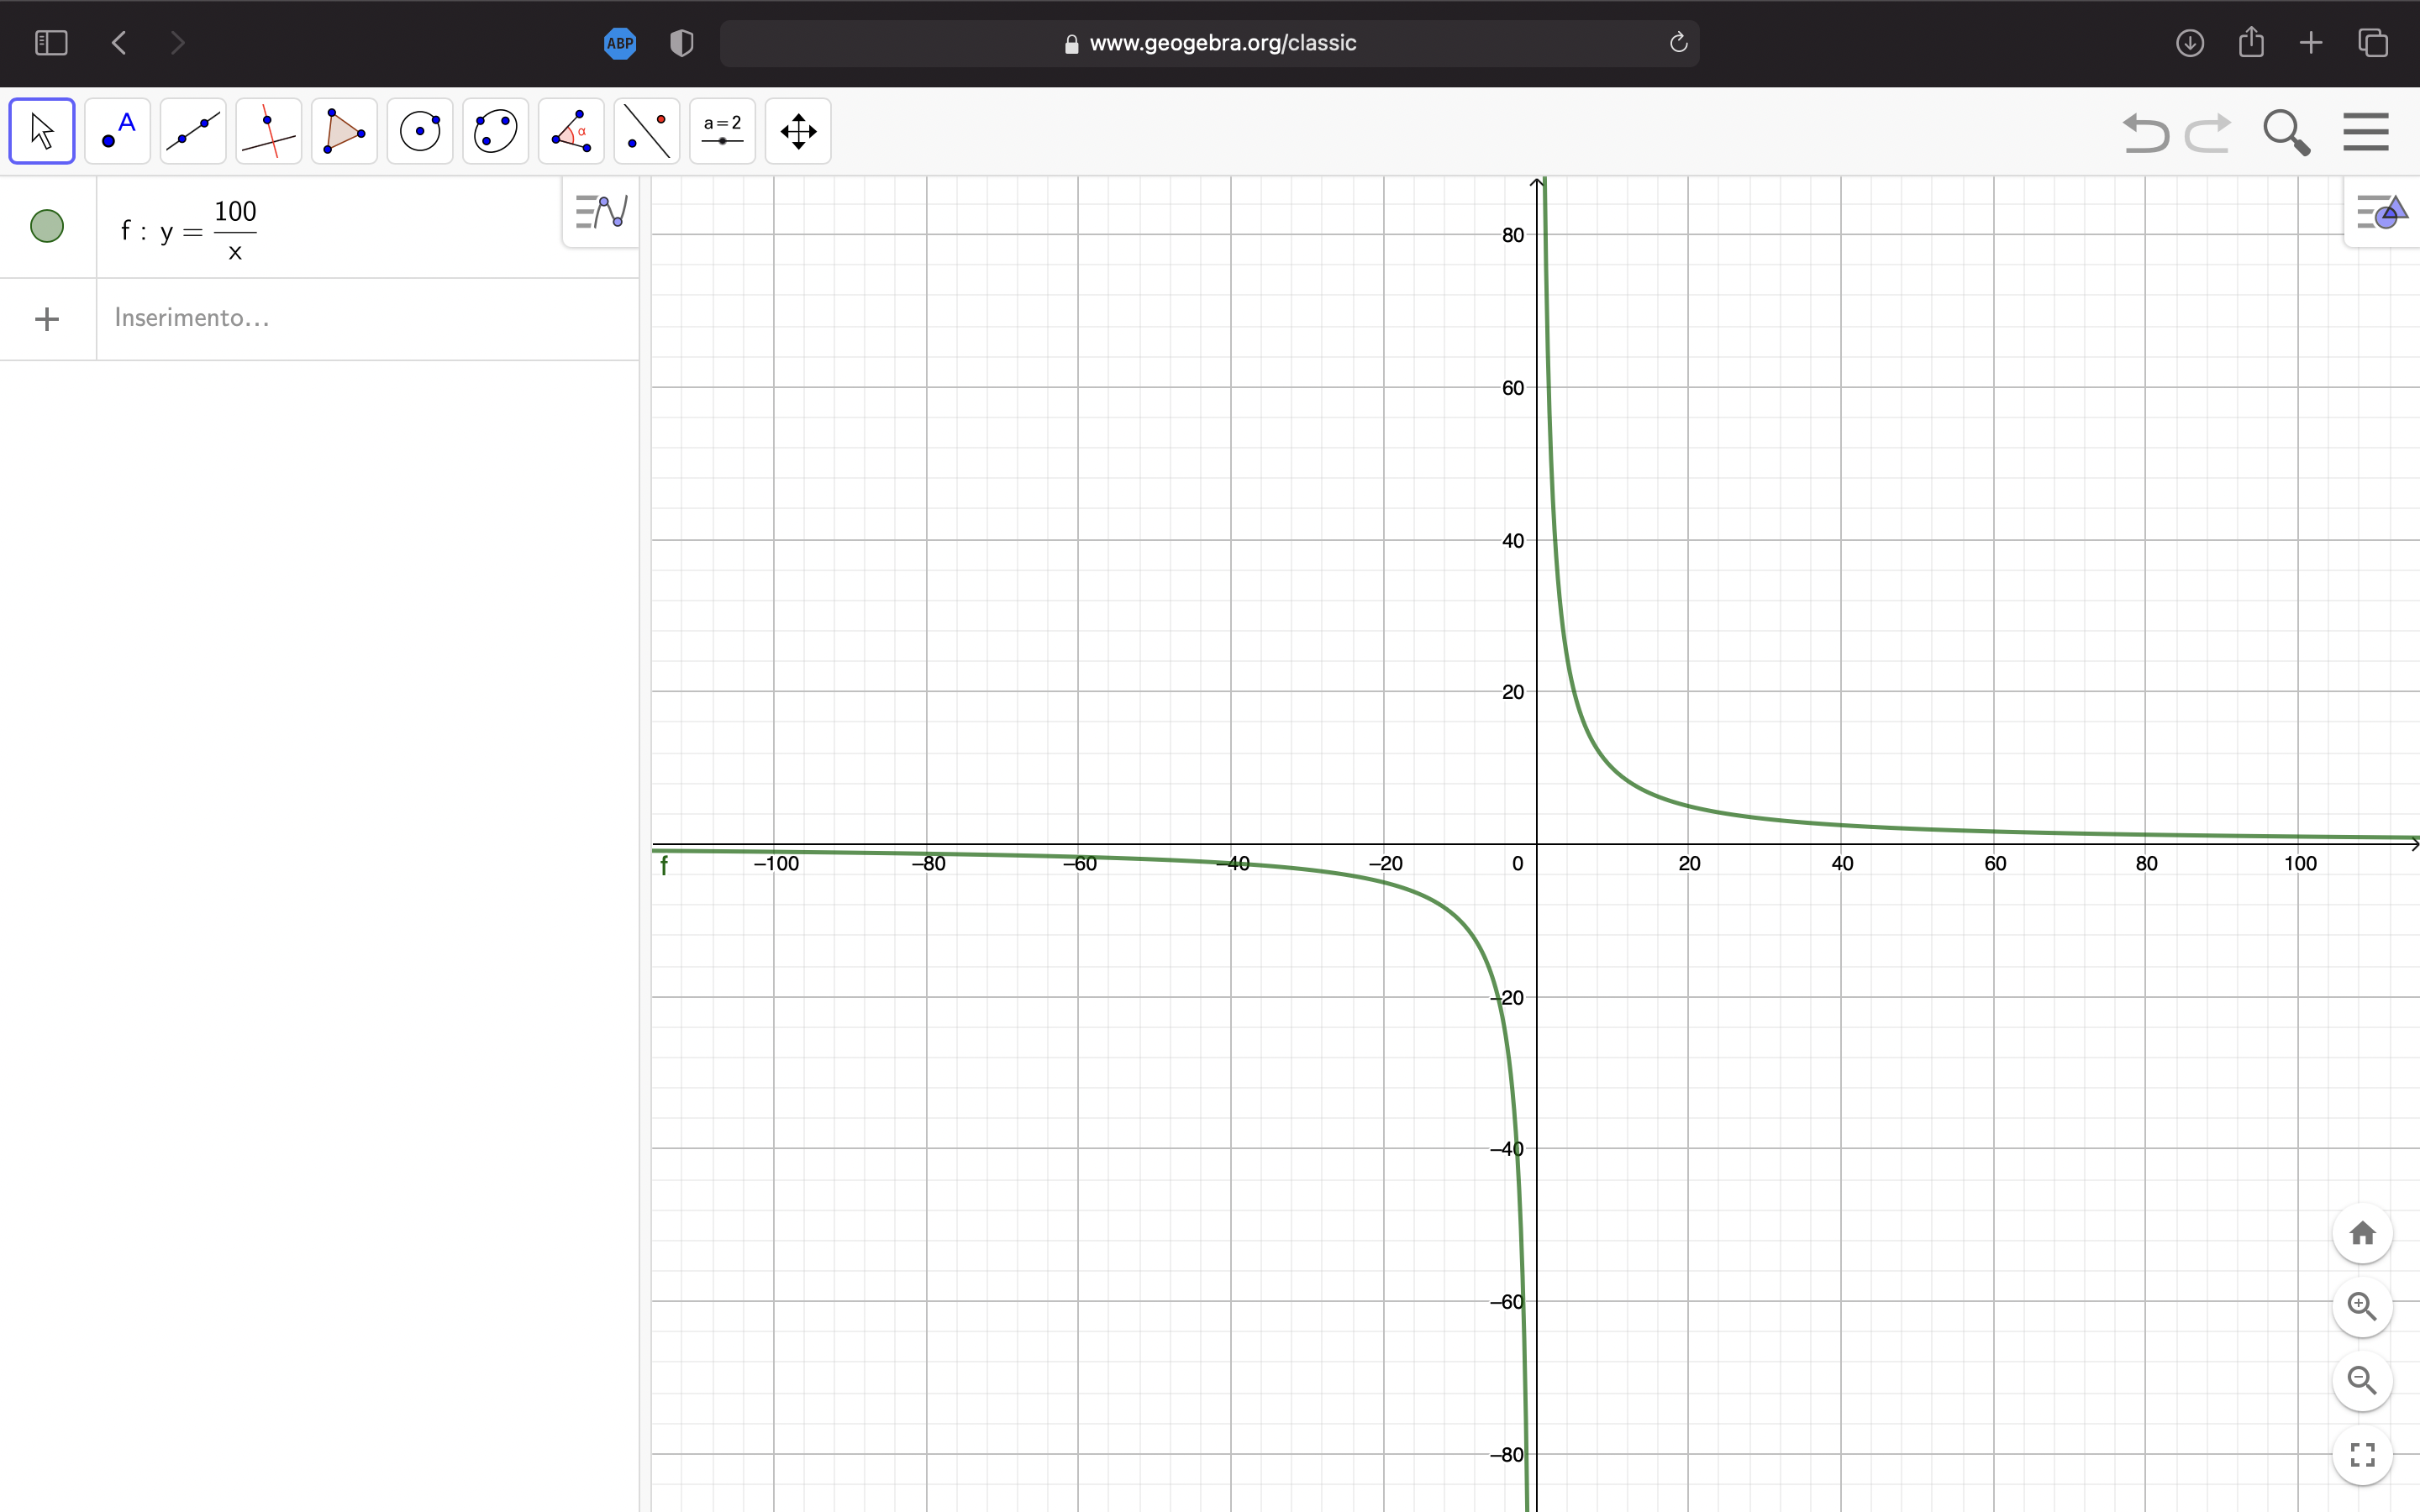
\includegraphics[scale=0.30]{100x}
    \end{center}
    \caption{L'andamento della funzione $100/x$}
    \label{fig: L'andamento della funzione $100/x$}
\end{figure}

La fitness di un determinato individuo, al contrario di quanto accade in altri tipi di algoritmi genetici, viene calcolata effettuando la \textbf{media aritmetica} della fitness di ogni gene all'interno dell'individuo. 
\newpage
\section{Operatori genetici}
  Verranno ora illustrate le scelte che sono state prese riguardo l'implementazione dei vari operatori genetici che prendono parte al processo di evoluzione tipico degli algoritmi genetici. Tutte le metodologie introdotte in questa sezione sono state presentate nella sesta lezione del corso di \textit{Fondamenti di Intelligenza Artificiale} tenuta dal Prof. \textbf{Fabio Palomba} e dal Dott. \textbf{Emanuele Iannone} nell'anno 2020.

    \subsection{L'operatore genetico di Selezione}
        Il primo operatore che viene applicato in una singola iterazione dell'algoritmo è quello di \textbf{selezione}, che, riprendendo quanto descritto in precedenza, permette di stabilire a quali individui sia concesso riprodursi sulla base della loro fitness. In letteratura, esistono diversi approcci che possono essere seguiti per realizzare quest'operazione. \\
        Tra questi vanno menzionati in particolare:

        \begin{itemize}
            \item L'approccio basato su \textbf{roulette wheel}, in cui gli individui con la fitness più alta hanno più possibilità di sopravvivere, proprio come succede ad un elemento posto su una roulette che ha una porzione di area maggiore rispetto agli altri. In questo caso, la "porzione" di roulette dedicata ad ogni individuo sarà direttamente proporzionale al valore della sua fitness (normalizzata in $[0, 1]$);
            \item L'approccio basato su \textbf{rank}, nel quale si effettua un ordinamento totale degli individui sulla base della loro fitness e ad ogni posizione in questa lista viene associato un numero, il cosiddetto \textit{rango}: la probabilità di selezione del singolo risulta inversamente proporzionale al suo rango;
            \item L'approccio basato su \textbf{truncation}, in qualche modo simile al precedente (ne mutua l'ordinamento degli individui) che consiste nel fissare un numero $n$ < $|P|$ (se P rappresenta la popolazione) e di selezionare i primi $n$ individui nella popolazione che hanno la fitness più alta.
        \end{itemize}

        Per l'algoritmo utilizzato in \textsc{ShallWeGo} si è scelto di utilizzare l'approccio basato su \textbf{roulette wheel} in quanto risulta quello di più immediata comprensione ed implementazione (essendo molto più fedele a quanto avviene in natura). Inoltre, non essendoci alcun caso in cui la fitness possa scendere sotto il valore $0$ quest'approccio è stato applicabile senza problemi.

    \subsection{L'operatore genetico di Crossover}
        Dopo l'applicazione dell'operatore di selezione (e quindi con la definizione di quelli che sono i componenti del cosiddetto \textbf{mating pool}), si procede con la fase di \textbf{crossover}, che prevede l'accoppiamento di coppie di individui all'interno del mating pool. 
        Esistono diverse tecniche che permettono di implementare questa operazione. \\
        Tra queste si menzionano:

        \begin{itemize}
            \item La tecnica \textbf{Single Point} che dati due individui x = ($x_{0}, x_{1}, ..., x_{n}$) ed y = ($y_{0}, y_{1}, ..., y_{m}$), prevede la creazione di due nuovi individui $j$ e $k$ che siano il risultato di un incrocio tra i geni dei loro genitori, dopo aver selezionato il cosiddetto \textbf{punto di taglio}, ovvero quel punto $z$ tale che:
                \begin{itemize}
                    \item $j = x_{0}, x_{1}, ..., x_{z}, y_{z+1}, ..., y_{m}$ e
                    \item $k = y_{0}, y_{1}, ..., y_{z}, x_{z+1}, ..., x_{n}$
                \end{itemize}
            \item La tecnica \textbf{\textit{k}-points}, che rappresenta una generalizzazione della tecnica Single Point, in cui un individuo viene diviso in \textit{$k$} porzioni prima di essere incrociato con un altro individuo;
        \end{itemize}
        La tecnica usata da \textsc{ShallWeGo} è quella del \textbf{Single Point}. C'è da precisare che nel caso del problema che si sta affrontando la posizione di un gene all'interno di un individuo risulta irrilevante e di conseguenza un approccio k-points non avrebbe portato a nessun tipo di miglioramento.
    \subsection{L'operatore genetico di Mutazione}
        L'ultimo operatore genetico che viene applicato durante un'iterazione è quello di \textbf{mutazione} che ricalca, come accennato precedentemente, il processo di mutazione spontanea che avviene in natura. Una mutazione consiste nel cambiamento casuale di un gene all'interno di un individuo. Anche in questo caso, esistono diversi approcci che in generale possono essere seguiti. \\
        Tra questi si menzionano:
        \begin{itemize}
            \item La tecnica del \textbf{Bit Flip} che, come suggerisce il nome, è applicabile solo nel caso di individui codificati in modo \textit{binario} e consiste nel scegliere in maniera casuale un gene all'interno dell'individuo e "capovolgere" il suo valore (quindi da 0 si passa ad 1 e viceversa);
            \item La tecnica del \textbf{Random Resetting} che prevede il cambiamento di un gene preso casualmente all'interno dell'individuo con un altro valore ammissibile per quel gene preso altrettanto casualmente;
            \item La tecnica dello \textbf{Swap} che prevede lo scambio di due geni all'interno dell'individuo;
            \item La tecnica dello \textbf{Scramble} che prevede una permutazione dei geni all'interno di un individuo.
        \end{itemize}

        La maggior parte di questi approcci risultano piuttosto rilevanti in un contesto in cui la posizione di un gene cambia la sua rilevanza del suo valore in un individuo, come nel caso di codifiche binarie (il bit più a sinistra, se posto ad 1, aumenta il valore decimale della stringa binaria che codifica l'individuo). \\
        Data la particolare natura del problema che si sta affrontando, non è possibile andare ad utilizzare la tecnica del Bit Flip e, allo stesso modo, le tecniche di Swap e Scramble non sono rilevanti in quanto la codifica dell'individuo non risente della posizione di un gene in particolare. \\
        Di conseguenza, la strategia che viene usata per questo algoritmo è quella del \textbf{Random Resetting}. In particolare, scelto un utente che è presente all'interno di un individuo, lo si sostituisce con un nuovo utente preso dal pool dei potenziali verificatori. Nel caso il nuovo utente che ha sostituito il precedente fosse già presente all'interno dell'individuo, il processo si ripete fino a non avere utenti duplicati.
        \newpage
\section{Termine del processo ed accorgimenti adottati}

    \subsection{Condizione di terminazione}
        L'algoritmo termina quando si verifica una delle seguenti tre condizioni:

        \begin{itemize}
            \item Vengono superate le 25 iterazioni del processo;
            \item Viene superato il limite di tempo stabilito (nel caso dell'algoritmo della piattaforma, quest'ultimo è fissato a 5 minuti);
            \item Per tre iterazioni consecutive la fitness della popolazione è minore rispetto a quella della miglior popolazione creata fino a quel momento.
        \end{itemize}

        Una condizione di terminazione impostata in questo modo contribuisce alla velocità dell'esecuzione dell'algoritmo, proprietà che è stata tenuta in grande considerazione in fase di progettazione della piattaforma.

        \subsection{La strategia dell'archivio}
            Come ulteriore accorgimento nello sviluppo dell'algoritmo, è stata implementata la cosiddetta \textbf{strategia dell'archivio} che consiste nel conservare una popolazione separata che non evolve composta da individui particolarmente forti, che si va a costruire man mano che le iterazioni vanno avanti. Nel caso specifico di \textsc{ShallWeGo} si è provveduto, per ogni iterazione, a tenere traccia del miglior individuo in termini di fitness della popolazione risultante dall'applicazione di ognuno dei tre operatori genetici. Il migliore tra questi tre verrà quindi aggiunto all'archivio.
            Essendo costituito da individui "forti", l'archivio può essere usato come alternativa alla popolazione che viene restituita dopo il termine della computazione dell'algoritmo. Questo, infatti, è proprio l'approccio scelto per la piattaforma: se al termine del processo la popolazione risultante avrà una fitness media minore o uguale a quella dell'archivio, la popolazione restituita sarà sostituita da quest'ultimo. \\
            La popolazione restituita sarà quindi soggetta a delle operazioni di postprocessing, illustrate di seguito.

        \subsection{Postprocessing}
            Il risultato dell'algoritmo consiste in una popolazione di individui, a loro volta composta da un gruppo di utenti. In precedenza, è stato specificato come la fitness di un individuo sia calcolata tramite una media aritmetica della fitness calcolata sui singoli geni. Si sfrutta quindi questa possibilità per effettuare un lavoro di post-processing sulla popolazione risultato. In particolare, si è scelto di effettuare le seguenti operazioni:

            \begin{itemize}
                \item Si ordinano gli individui in maniera decrescente in base alla loro fitness;
                \item Si ottiene, a partire dal singolo individuo, la lista degli utenti che esso contiene, ordinati in maniera decrescente rispetto al loro valore di fitness;
                \item Per ognuna di queste liste, viene preso il primo utente. Ci si ferma quando sono stati considerati tutti gli individui o quando sono stati presi 5 utenti. Il risultato di questa operazione sarà di fatto un nuovo insieme di utenti formato da quelli più "forti" tra quelli presenti negli individui della popolazione risultante dall'algoritmo.
            \end{itemize}

            Sebbene le operazioni di post processing (trattandosi prettamente di ordinamento) assumano una complessità di almeno $\mathcal{O}(n\log{}n)$, esse vengono effettuate su un dominio particolarmente più piccolo rispetto a quello dei candidati (che mettendosi nel contesto di una piattaforma ben avviata potrebbero essere in numero molto elevato o comunque tale da rendere la ricerca esaustiva poco efficiente) e che allo stesso tempo permettono di ottenere un risultato ancora migliore rispetto a quello ottenuto con la semplice evoluzione, riuscendo cioè a creare un gruppo di utenti che risultino "forti tra i forti" in termini di fitness assoluta. Ciò giustifica la presenza sia della procedura di evoluzione degli individui sia il postprocessing. \\ 
            Le operazioni di ordinamento non richiedono un ulteriore calcolo della fitness in quanto in fase di implementazione è stato effettuato il caching di quel valore per quella determinata istanza dell'algoritmo e sicuramente questo valore alla fine sarà già stato calcolato e conservato, riducendo il calcolo finale della fitness ad un semplice accesso ad una variabile che non richiede operazioni particolari.


    \subsection{Risultati dell'algoritmo con i parametri correnti}
        Nella sua fase di testing, l'algoritmo è stato eseguito su un insieme molto grande di utenti generato in maniera casuale (un utente per ogni comune e con fitness presa casualmente tra 0 e 65). Nella tabella che segue sono riportati i risultati dell'algoritmo su diverse istanze. In particolare, 

        \begin{itemize}
            \item Nella \textbf{prima colonna} è riportato il Comune della segnalazione;
            \item Nella \textbf{seconda colonna} sono riportati Comune di residenza e livello di karma degli utenti selezionati dall'algoritmo per verificare quella determinata segnalazione, dopo l'applicazione del post-processing.
        \end{itemize}

        \begin{center}

            \begin{table}[H]
                \centering
                \begin{tabular}{|l|l|}
                \hline
                Fisciano         & \begin{tabular}[c]{@{}l@{}}Cava de' Tirreni (karma: 48.6)\\ Siano (karma: 12.5)\\ Baronissi (karma: 17.8)\\ Roccapiemonte (karma: 47.8)\\ Trentinara (karma: 53.6)\end{tabular}                                          \\ \hline
                Nocera Inferiore & \begin{tabular}[c]{@{}l@{}}Nocera Inferiore (karma: 29.2)\\ Sant'Egidio del Monte Albino (karma: 39.3)\\ San Marzano sul Sarno (karma: 53.4)\\ Roccapiemonte (karma: 47.8)\\ Nocera Superiore (karma: 24.2)\end{tabular} \\ \hline
                Salerno          & \begin{tabular}[c]{@{}l@{}}Giffoni Sei Casali (karma: 45.3)\\ Pontecagnano Faiano (karma: 44.2)\\ Baronissi (karma: 17.8)\\ Laviano (karma: 46.8)\\ Maiori (karma: 46.6) \end{tabular}                                   \\ \hline
                \end{tabular}
                \caption{\label{tab:table-name}Risultati dell'algoritmo su diversi input.}
                \end{table}
        \end{center}

        Si noti come nel caso dell'istanza dell'algoritmo per la città di Nocera Inferiore sia presente un utente che opera proprio in quel comune: egli rappresenta quindi parte della soluzione ottima. Nel caso della città di Salerno, invece, è stato incluso un utente la cui distanza dal luogo della segnalazione si aggira attorno ai 47km in linea d'aria (Laviano). Quest'utente è stato incluso nella soluzione in virtù del proprio valore di \textit{karma} che risulta discretamente alto. 
        

\newpage
